% Appendix A

\chapter{Batches fabrication and hardness/density measurements details} % Main appendix title

\label{AppendixA} % For referencing this appendix elsewhere, use \ref{AppendixA}

\section{Process parameters and measured hardness/density properties}
\label{ppa}
All manufacturing set values are gathered in table \ref{table:Pparam}. Dimensions of the cubic, cylindrical and parallelepiped specimens are noted in accordance with figure \ref{fig:cc}.\\

 \begin{center}
%\begin{table}[ht]
\setlength\LTleft{-0.7in}
%\setlength\LTright{-1in}
\begin{landscape}
\begin{savenotes}

\begin{longtable}{@{\extracolsep{\fill}}*{12}{|c}|@{}}
    \hline
  Batch name & Contour & Type & Dimensions [mm] &Specimen name & $\frac{P}{P_{max}} [-]$ & $v_s [\frac{mm}{s}]$ & $E_d [\frac{J}{mm^3}]$ & $H_v [HV]$ & $\rho_{rel}$ \footnote{Measured by RODIA [\%].} & $\rho_{a,rel}$ \footnote{Measured by HW (AB specimens) [\%].} & $\rho_{a,rel}$ \footnote{Measured by HW (polished specimens) [\%].} \\
  \hline
  \hline
  \endfirsthead
\multicolumn{12}{c}%
{\tablename\ \thetable\ -- \textit{Continued from previous page}} \\
\hline
Batch name & Contour & Type & Dimensions [mm] &Specimen name & $\frac{P}{P_{max}} [-]$ & $v_s [\frac{mm}{s}]$  & $E_d [\frac{J}{mm^3}]$ & $H_v [HV]$ & $\rho_{rel}$  & $\rho_{a,rel}$  & $\rho_{a,rel}$ \\
\hline
\endhead

\hline \multicolumn{12}{c}{\textit{Continued on next page}} \\
\caption[Manufacturing process parameters]{Manufacturing process parameters}
\label{table:Pparam}

\endfoot
\hline
\endlastfoot

  X200-171024 & No & Cubic & L=10& 1 & 0.85 & 900 & & & & &\\
  & &   & & 2 &  & 1000 & & & & &\\
  & &   & & 3&  & 1059& & & & &\\
  & &  & & 4&  & 1500& & & & &\\
  & &  & & 5& 1 & 900& & & & &\\
  & &  & & 6&  & 1059& & & & &\\
  & & & & 7 & 0.75 & 1200& & & & &\\
  & & & & 7a & & & & & & &\\
  & & & & 7b & & & & & & &\\
  & & & & 8& & 900& & & & &\\
    & & & & 8a & & & & & & &\\
      & & & & 8b & & & & & & &\\
\hline  
  X200-180109 & No&Cubic & L=10 & 7c & 0.75 &1200 & & & & &\\
  & & & & 7d & & & & & & &\\
  & & & & 7e & & & & & & & \\
  & & & & 7f & & & & & & &\\
  & & & & 7g & & & & & & &\\ 
  & & & & 7h & & & & & & &\\        
  & & & & 7i & & & & & & &\\        
  & & & & 7j & & & & & & &\\        
  & & & & 7k & & & & & & &\\        
  & & & & 7l & & & & & & &\\      
  & & & & 7m & & & & & & &\\      
  & & & & 7n & & & & & & &\\
  & & & & 7o & & & & & & &\\
  & & & & 7p & & & & & & &\\
  & & & & 7q & & & & & & &\\                    
  & & & & 8c& & 900 & & & & &\\
  & & & & 8d & & & & & & &\\
  & & & & 8e & & & & & & &\\
  & & & & 8f & & & & & & &\\
  & & & & 8g & & & & & & &\\
  & & & & 8h & & & & & & &\\
  & & & & 8i & & & & & & &\\
  & & & & 8j & & & & & & &\\
  & & & & 8k & & & & & & &\\  
  & & & & 8l & & & & & & &\\
  & & & & 8m & & & & & & &\\
  & & & & 8n & & & & & & &\\
  & & & & 8o & & & & & & &\\     
  & & & & 8p & & & & & & &\\
  & & & & 8q & & & & & & &\\        
\hline  
  X200-180220 & No & Cubic & L=5 & TT150-2 & 0.75 & 1200 & & & & &\\
  & &  & & TT200-2 &  & & & & & &\\
  & &  & & TT300-2 &  & & & & & &\\
  & &  & & TT300-2-plaque &  & & & & & &\\
  & &  & & TT150-2-real &  & & & & & &\\
  & &  & & TT200-2-real &  & & & & & &\\
  & &  & & TT250-2-real &  & & & & & &\\
  & &  & & TT300-2-real &  & & & & & &\\
\hline  
  X200-180222 & No & Cubic & L=10 &12& 0.75 & 1200\\
  & &  & &13 &  & & & & & &\\
\hline  
  X200-180228  & Yes & Cylindrical & D=6, H=2 &1 & 0.75 & 1200 & & & & &\\
  & &  &  & 2&  & & & & & &\\
  & &  &  & 3 &  & & & & & &\\
\hline  
  X200180313 & Yes & Cylindrical & D=6, H=10&1& 0.75 & 1200 & & & & &\\
    & &    & &2 & & & & & & & \\
    & &  &D=12, H=10 &3& & & & & & & \\
    & & & &4 & & & & & & &\\
    & No & Parallelepiped & H=10, W=40, L=120 & ??? & & & & & & &\\
        &  & & & ??? & & & & & & &\\
\hline  
  X200-180315 & No & Parallelepiped & H=10, W=40, L=115& ??? & 0.75 & 1200 & & & & &\\
  \hline
  X200-180319  & No & Cubic & L=10 & cub 1 & 0.75 & 1200 & & & & &\\
  & &  & & cub 2 & & & & & & &\\
  & &  & & cub 3 & & & & & & &\\
  & & & & cub 4 & & & & & & &\\
  & & & & cub 5 & & & & & & &\\
  & & &  L=5& TT300-1-real &  & & & & & &\\ 
  & Yes &  Cylindrical & D=6, H=10&cyl 1   &  & & & & & &\\
    & &  & &cyl 2 & & & & & & &\\
    & &  & D=12, H=10 &cyl 3 & & & & & & &\\
    & &  &  &cyl 4  & & & & & & &\\
 & No & Parallelepiped & H=10, W=40, L=120 & ??? & & & & & & &\\ 
    \hline 
X200-180417 & Yes & Tensile & (see section \ref{MMFPP}) & 1, ..., 25 & 0.75 &1200 & & & & &\\
& No &  & & 26, 27, 28 & && & & & &\\
&  & Cubic & L=10 & A & && & & & &\\
&  & & & B & && & & & &\\
&  & & & C & && & & & &\\
\end{longtable}
\end{savenotes}
\end{landscape}
%\end{table}
 \end{center}

\section{Specimens positioning, fabrication orders and sintering times}
\label{mda}
\subsection{Batch X200-171024}

\begin{figure}[ht]
\centering
\noindent\makebox[\textwidth]{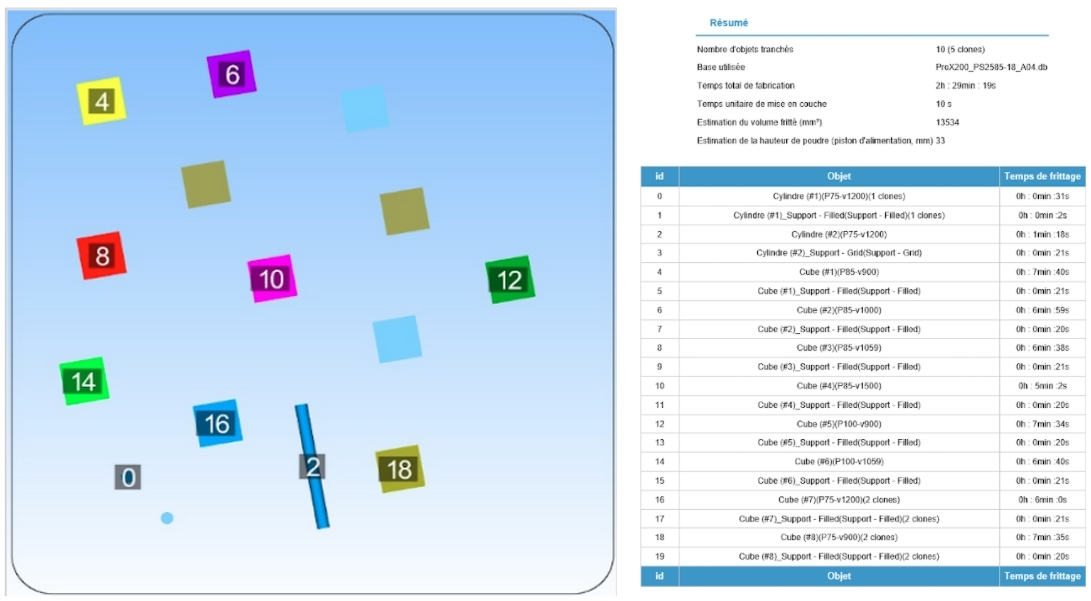
\includegraphics[scale=0.58]{Images/171024-cad}}
\decoRule
\caption[Specimens positions, order of fabrication and sintering times for batch X200-171024]{Specimens positions, order of fabrication and sintering times for batch X200-171024}
\label{fig:171024-cad}
\end{figure}

\begin{figure}[ht]
\centering
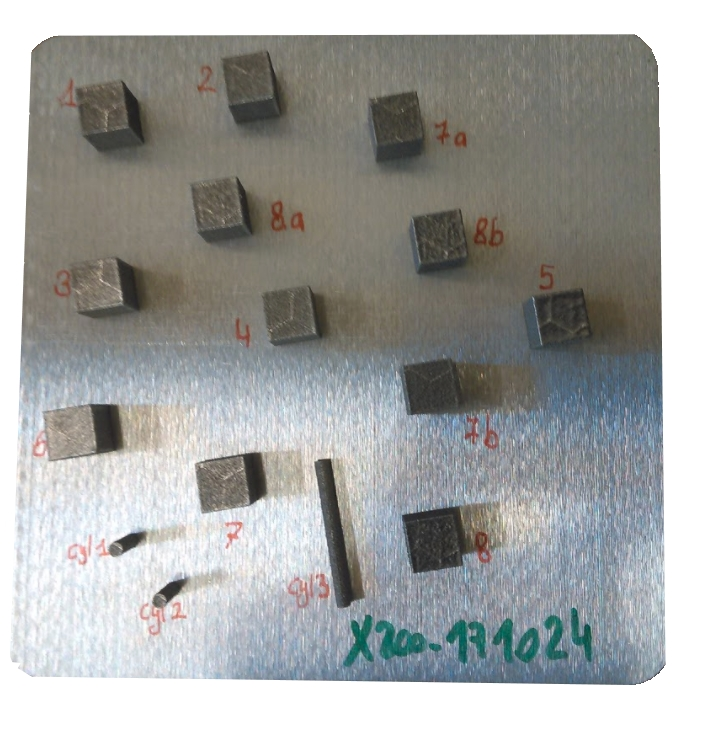
\includegraphics[scale=0.45]{Images/171024-real}
\decoRule
\caption[Photography of the manufacturing plate after completion of the fabrication of batch X200-171024]{Photography of the manufacturing plate after completion of the fabrication of batch X200-171024}
\label{fig:171024-real}
\end{figure}


\subsection{Batch X200-180109}

\begin{figure}[ht]
\centering
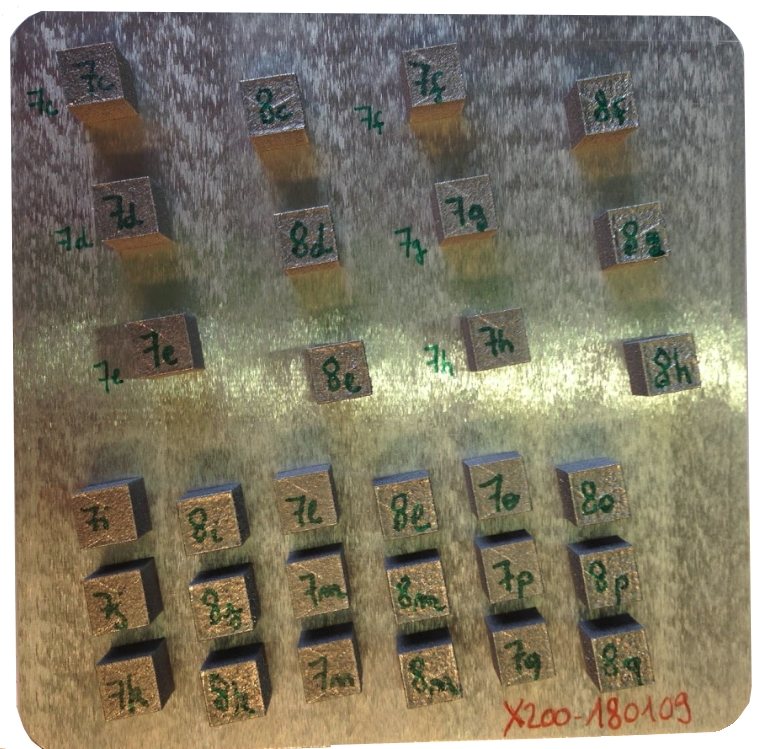
\includegraphics[scale=0.45]{Images/180109-real}
\decoRule
\caption[Photography of the manufacturing plate after completion of the fabrication of batch X200-180109]{Photography of the manufacturing plate after completion of the fabrication of batch X200-180109}
\label{fig:180109-real}
\end{figure}

\subsection{...Other batches}